\documentclass{article}

\usepackage[load-configurations = abbreviations]{siunitx}
\usepackage{graphicx}

\title{Analysis of Coupled Oscillators through Fourier Methods}
\author{Raymond Langehennig}

\begin{document}
\maketitle

\begin{abstract}
    test
\end{abstract}

\section{Introduction}

\subsection{Coupled and driven oscillators}
When a system exhibiting oscillatory motion (an oscillator) is subjected to a periodic, external force, it is known as a \emph{driven oscillator}. Driven oscillators exhibit a behavior known as \emph{resonance} when the frequency of the external force matches the oscillatory frequency of the system, at which point the amplitude of oscillation may increase dramatically, depending on how damped the system is.

A \emph{coupled oscillator} is a system with multiple oscillatory elements that influence each other in some way. This could be something like two pendulums connected by a spring, or the atoms of a metal connected by electromagnetism. For such a system, an arbitrary displacement from equilibrium usually results in complicated motion where the frequency at which each element oscillates itself continuously oscillates; however, coupled oscillators are capable of certain so-called \emph{normal modes} of motion, where each element oscillates at the same, fixed frequency. This can be seen in the example of the two spring-coupled pendulums, for instance, which has two normal modes: the first when the two pendulums are given the same initial displacement in the same direction, and the second when they are given the same displacement but in opposite directions. When a coupled oscillator is driven, resonance may be achieved at the frequency of any one of these normal modes.

\subsection{Objective}
The subject of study in this report is a magnetically coupled, magnetically driven, torsional oscillator, and the object is to observe and analyze its motion with an oscilloscope and ultimately a fast Fourier transform spectrum analyzer, in order to find the frequencies of the normal modes.

\begin{figure}
    \centering
    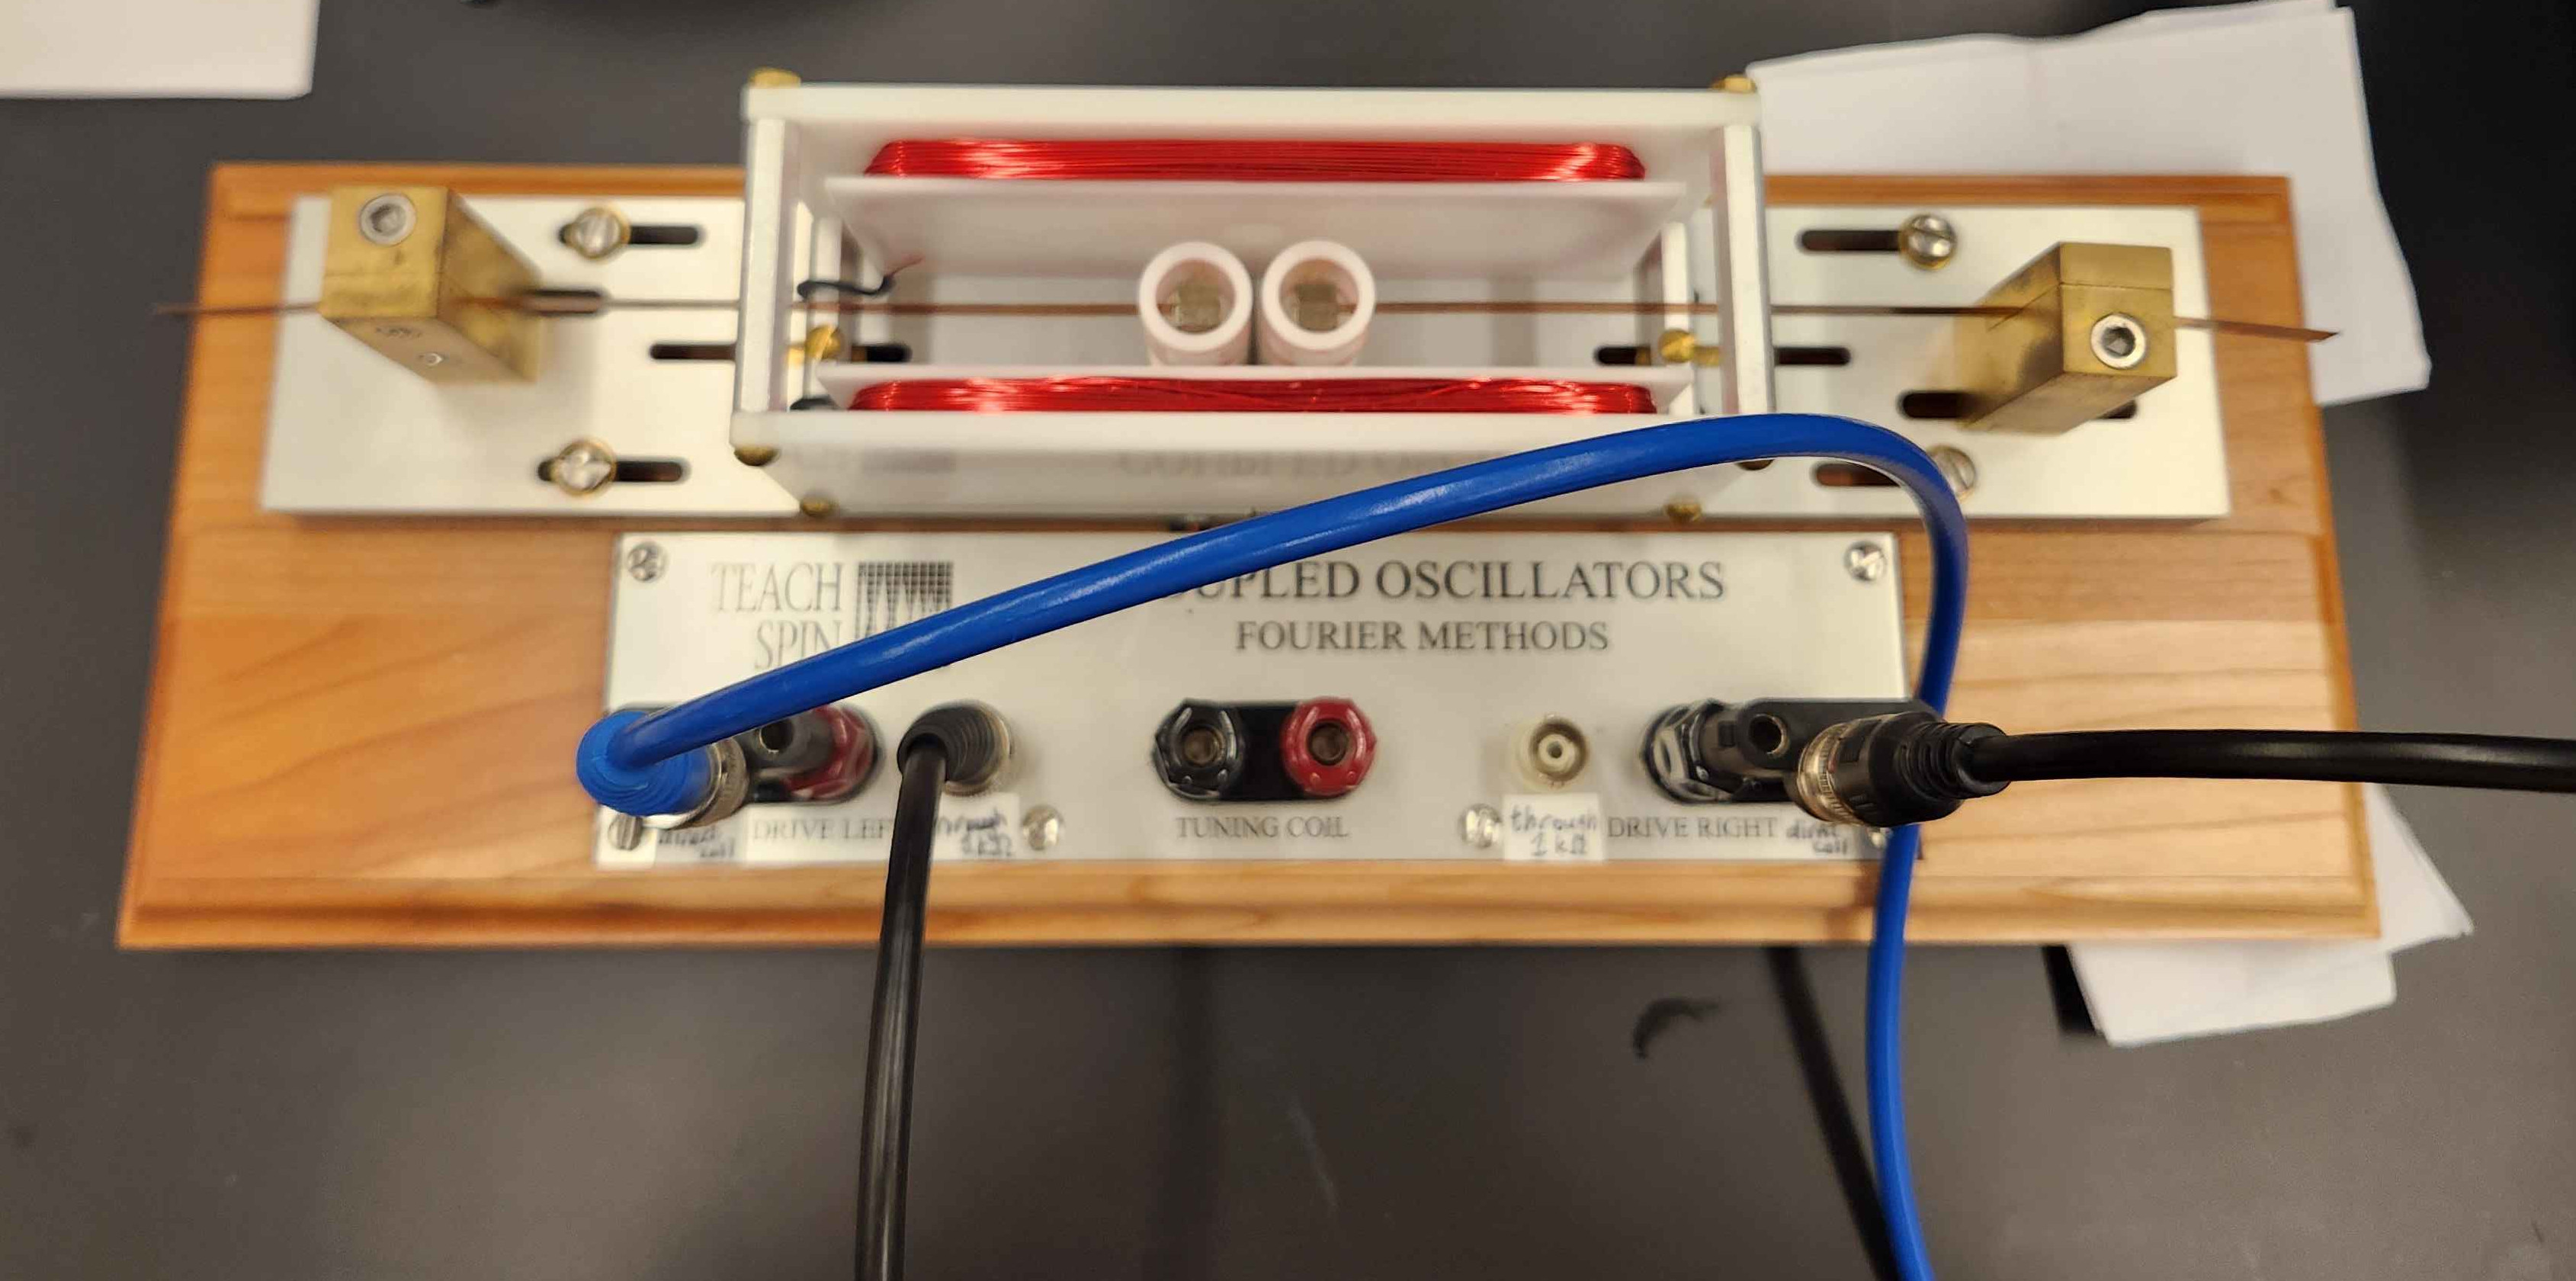
\includegraphics[width=0.5\linewidth]{20250910_113924.jpg}
    \caption{Photo of the torsional oscillator used.}
\end{figure}

\subsection{Model}
The oscillator consists of two phosphor-bronze reeds in-line with each other, clamped on the outer ends and with a magnetic neodymium cube on the inner ends. These magnets are placed inside vertical coils that allow for either excitation or detection, and both reeds are placed inside horizontal coils meant for tuning the entire system.

The resonant frequency of a single reed can be calculated easily by $\omega = \sqrt{\kappa/I}$. $\kappa$ may be calculated using \[ \kappa = G\frac{wt^3}{3L}, \] where $G = \qty{41}{\giga\pascal}$ is the shear modulus, $w = \qty{6.35}{\mm}$ is the width of the reed, $t = \qty{0.254}{\mm}$ is the thickness or depth of the reed, and $L = \qty{100}{\mm}$ is the length of the reed, all giving $\kappa \approx \qty{0.014}{N.m}$. The rotational inertia of the cube $I = \rho\ell^5/6 \approx \qty{0.129}{\gram.\cm^2}$, with a density $\rho = \qty{7.51}{g/cm^3}$ and side length $\ell = \qty{6.35}{mm}$. This gives $\omega = \qty{1049.04}{\per\s}$ and therefore a $f = \qty{167}{Hz}$


\section{Materials and Procedure}


\section{Results}
\subsection{Raw data}
\subsection{Processed data}

\section{Conclusion}

\end{document}
